   \documentclass{article}
\usepackage{pgfplots}
\begin{document}
\begin{figure}
\centering

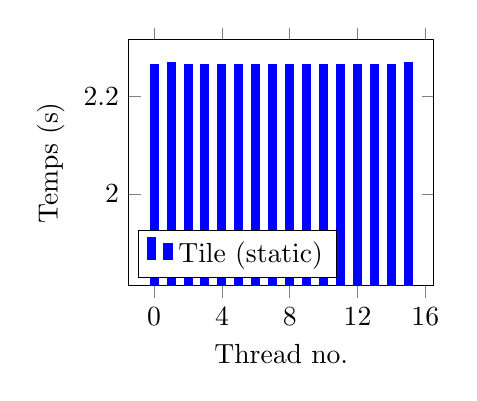
\begin{tikzpicture}
\begin{axis}[
  ybar,
  bar width=0.1cm,
  xlabel={Thread no.},
  ylabel={Temps (s)},
  ymin=1.811627,
  legend pos=south west,
  width=0.45\textwidth,
  xtick distance=4
]

% Données pour le premier graphique (à gauche)
\addplot[color=blue, fill=blue] coordinates {
  (0,2.264657) (1,2.270237) (2,2.264941) (3,2.266108) (4,2.264658) (5,2.264568) (6,2.264537) (7,2.264560) (8,2.264552) (9,2.264583) (10,2.264534) (11,2.264890) (12,2.264587) (13,2.264877) (14,2.264886) (15,2.270256)
};
\addlegendentry{Tile (static)}

\end{axis}
\end{tikzpicture}
\hfill
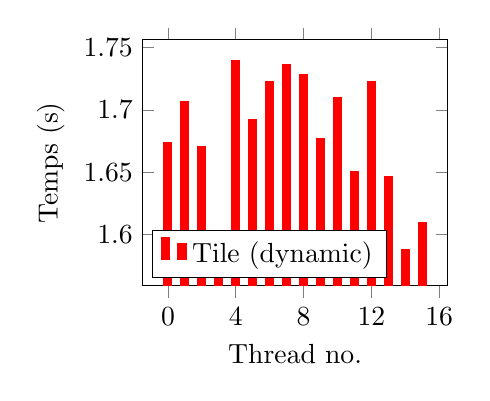
\begin{tikzpicture}
\begin{axis}[
  ybar,
  bar width=0.1cm,
  xlabel={Thread no.},
  ylabel={Temps (s)},
  ymin=,
  legend pos=south west,
  width=0.45\textwidth,
  xtick distance=4
]

% Données pour le deuxième graphique (au milieu)
\addplot[color=red, fill=red] coordinates {
  (0,1.673452) (1,1.706398) (2,1.670358) (3,1.575347) (4,1.739719) (5,1.691898) (6,1.722376) (7,1.736459) (8,1.727955) (9,1.676728) (10,1.709942) (11,1.650857) (12,1.722343) (13,1.646555) (14,1.587996) (15,1.609344)
};
\addlegendentry{Tile (dynamic)}

\end{axis}
\end{tikzpicture}
\hfill
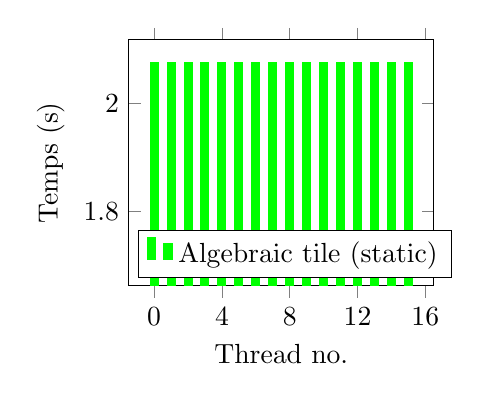
\begin{tikzpicture}
\begin{axis}[
  ybar,
  bar width=0.1cm,
  xlabel={Thread no.},
  ylabel={Temps (s)},
  ymin=1.661708,
  legend pos=south west,
  width=0.45\textwidth,
  xtick distance=4
]

% Données pour le troisième graphique (à droite)
\addplot[color=green, fill=green] coordinates {
  (0,2.077175) (1,2.077136) (2,2.077182) (3,2.077166) (4,2.077173) (5,2.077184) (6,2.077163) (7,2.077228) (8,2.077217) (9,2.077191) (10,2.077173) (11,2.077180) (12,2.077191) (13,2.077157) (14,2.077164) (15,2.077217)
};
\addlegendentry{Algebraic tile (static)}

\end{axis}
\end{tikzpicture}

\caption{Temps d'exécution des threads pour le fichier gemm.c}
\label{fig:graphes}
\end{figure}

\begin{table}[htbp]
  \centering
  \caption{Statistiques pour le fichier gemm.c}
  \begin{tabular}{|c|c|c|c|}
    \hline
    Statistique & Algebraic Tile & Tile (static) & Tile (dynamic) \\ 
    \hline
    Skewness (g1)  & 0.386377 & 2.10998 & -0.674585 \\ 
    Kurtosis (g2)  & -0.214553 & 2.67479 & -0.676126 \\ 
    Coefficient de variation $ \frac{\sigma}{\overline{x}} $ & 1.1171e-05 & 0.000814395 & 0.0301075\\ 
    Percent Imbalance metric en \% & 0.00231083 & 0.211701 & 3.67936\\ 
    Coefficient de Gini  & 6.12872e-06 & 0.000319186 & 0.0167496\\ 
    Temps d'exécution (s) &  2.077357    &  2.271536   &  1.741859   \\ 

    \hline
  \end{tabular}
\end{table}\newline
g1=$ \frac{\sum_{i=1}^{n} (x_i - \overline{x})^3}{n\sigma^3} $\
g2=$ \frac{\sum_{i=1}^{n} (x_i - \overline{x})^4}{n\sigma^4} $\
Coefficient de Gini = $ \frac{\sum_{i=1}^{n}\sum_{j=1}^{n} |x_i - x_j|}{2n^2\overline{x}} $\
\newpage

\begin{figure}
\centering

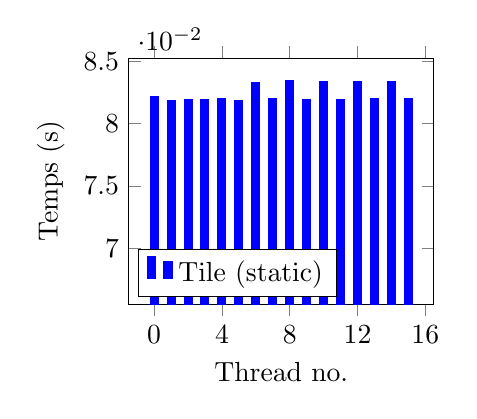
\begin{tikzpicture}
\begin{axis}[
  ybar,
  bar width=0.1cm,
  xlabel={Thread no.},
  ylabel={Temps (s)},
  ymin=.065492,
  legend pos=south west,
  width=0.45\textwidth,
  xtick distance=4
]

% Données pour le premier graphique (à gauche)
\addplot[color=blue, fill=blue] coordinates {
  (0,0.082172) (1,0.081866) (2,0.081946) (3,0.081942) (4,0.081997) (5,0.081885) (6,0.083330) (7,0.081986) (8,0.083478) (9,0.081917) (10,0.083420) (11,0.081929) (12,0.083406) (13,0.082032) (14,0.083418) (15,0.082063)
};
\addlegendentry{Tile (static)}

\end{axis}
\end{tikzpicture}
\hfill
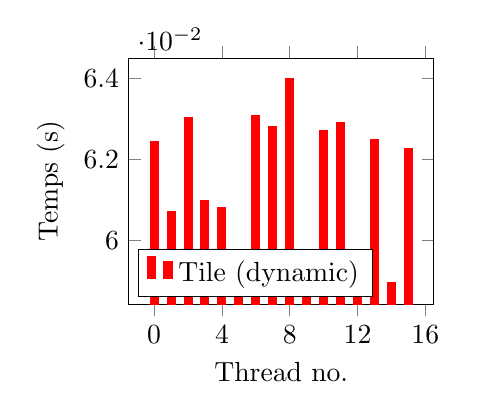
\begin{tikzpicture}
\begin{axis}[
  ybar,
  bar width=0.1cm,
  xlabel={Thread no.},
  ylabel={Temps (s)},
  ymin=,
  legend pos=south west,
  width=0.45\textwidth,
  xtick distance=4
]

% Données pour le deuxième graphique (au milieu)
\addplot[color=red, fill=red] coordinates {
  (0,0.062435) (1,0.060709) (2,0.063050) (3,0.060975) (4,0.060817) (5,0.058933) (6,0.063087) (7,0.062816) (8,0.064001) (9,0.059401) (10,0.062724) (11,0.062918) (12,0.059449) (13,0.062505) (14,0.058949) (15,0.062283)
};
\addlegendentry{Tile (dynamic)}

\end{axis}
\end{tikzpicture}
\hfill
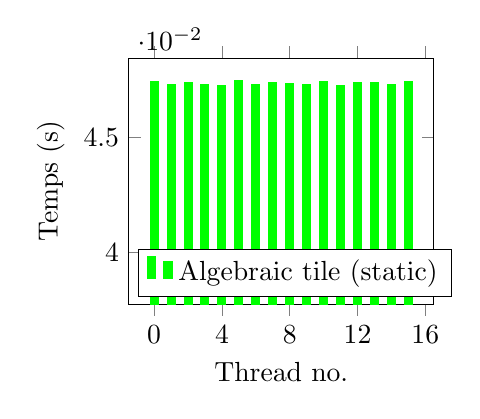
\begin{tikzpicture}
\begin{axis}[
  ybar,
  bar width=0.1cm,
  xlabel={Thread no.},
  ylabel={Temps (s)},
  ymin=.037777,
  legend pos=south west,
  width=0.45\textwidth,
  xtick distance=4
]

% Données pour le troisième graphique (à droite)
\addplot[color=green, fill=green] coordinates {
  (0,0.047406) (1,0.047284) (2,0.047367) (3,0.047299) (4,0.047241) (5,0.047454) (6,0.047265) (7,0.047372) (8,0.047304) (9,0.047270) (10,0.047424) (11,0.047222) (12,0.047379) (13,0.047355) (14,0.047293) (15,0.047412)
};
\addlegendentry{Algebraic tile (static)}

\end{axis}
\end{tikzpicture}

\caption{Temps d'exécution des threads pour le fichier gemver.c}
\label{fig:graphes}
\end{figure}

\begin{table}[htbp]
  \centering
  \caption{Statistiques pour le fichier gemver.c}
  \begin{tabular}{|c|c|c|c|}
    \hline
    Statistique & Algebraic Tile & Tile (static) & Tile (dynamic) \\ 
    \hline
    Skewness (g1)  & 0.0757661 & 0.780291 & -0.41236 \\ 
    Kurtosis (g2)  & -1.22205 & -1.33967 & -1.2473 \\ 
    Coefficient de variation $ \frac{\sigma}{\overline{x}} $ & 0.0014476 & 0.00811745 & 0.026292\\ 
    Percent Imbalance metric en \% & 0.253094 & 1.27851 & 3.95544\\ 
    Coefficient de Gini  & 0.000826487 & 0.00403074 & 0.0146058\\ 
    Temps d'exécution (s) &  0.047810    &  0.083879   &  0.064326   \\ 

    \hline
  \end{tabular}
\end{table}\newline
g1=$ \frac{\sum_{i=1}^{n} (x_i - \overline{x})^3}{n\sigma^3} $\
g2=$ \frac{\sum_{i=1}^{n} (x_i - \overline{x})^4}{n\sigma^4} $\
Coefficient de Gini = $ \frac{\sum_{i=1}^{n}\sum_{j=1}^{n} |x_i - x_j|}{2n^2\overline{x}} $\
\newpage

\begin{figure}
\centering

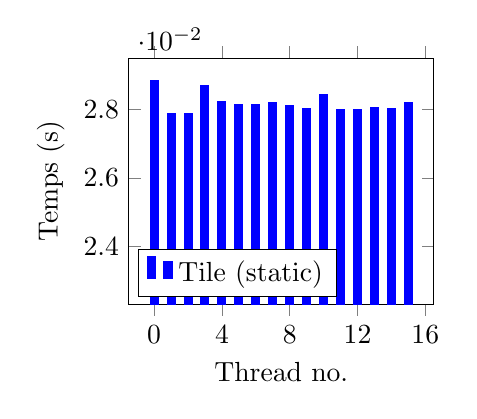
\begin{tikzpicture}
\begin{axis}[
  ybar,
  bar width=0.1cm,
  xlabel={Thread no.},
  ylabel={Temps (s)},
  ymin=.022302,
  legend pos=south west,
  width=0.45\textwidth,
  xtick distance=4
]

% Données pour le premier graphique (à gauche)
\addplot[color=blue, fill=blue] coordinates {
  (0,0.028857) (1,0.027878) (2,0.027880) (3,0.028721) (4,0.028233) (5,0.028148) (6,0.028153) (7,0.028203) (8,0.028128) (9,0.028039) (10,0.028438) (11,0.028013) (12,0.028017) (13,0.028070) (14,0.028032) (15,0.028200)
};
\addlegendentry{Tile (static)}

\end{axis}
\end{tikzpicture}
\hfill
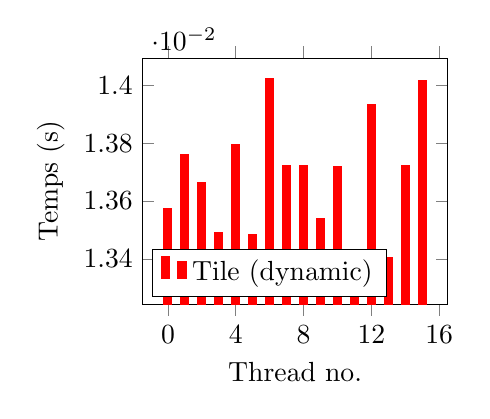
\begin{tikzpicture}
\begin{axis}[
  ybar,
  bar width=0.1cm,
  xlabel={Thread no.},
  ylabel={Temps (s)},
  ymin=,
  legend pos=south west,
  width=0.45\textwidth,
  xtick distance=4
]

% Données pour le deuxième graphique (au milieu)
\addplot[color=red, fill=red] coordinates {
  (0,0.013574) (1,0.013762) (2,0.013664) (3,0.013491) (4,0.013794) (5,0.013485) (6,0.014024) (7,0.013724) (8,0.013722) (9,0.013539) (10,0.013720) (11,0.013314) (12,0.013935) (13,0.013404) (14,0.013722) (15,0.014017)
};
\addlegendentry{Tile (dynamic)}

\end{axis}
\end{tikzpicture}
\hfill
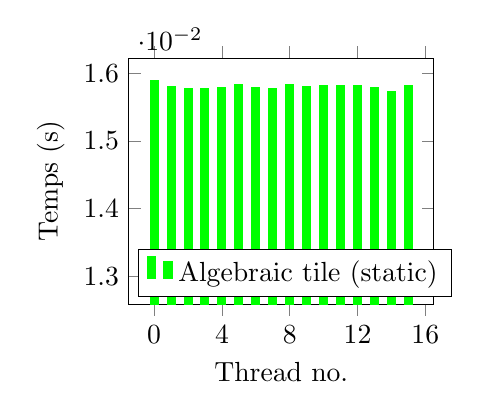
\begin{tikzpicture}
\begin{axis}[
  ybar,
  bar width=0.1cm,
  xlabel={Thread no.},
  ylabel={Temps (s)},
  ymin=.012588,
  legend pos=south west,
  width=0.45\textwidth,
  xtick distance=4
]

% Données pour le troisième graphique (à droite)
\addplot[color=green, fill=green] coordinates {
  (0,0.015893) (1,0.015797) (2,0.015777) (3,0.015773) (4,0.015789) (5,0.015831) (6,0.015792) (7,0.015767) (8,0.015834) (9,0.015810) (10,0.015821) (11,0.015816) (12,0.015819) (13,0.015782) (14,0.015735) (15,0.015813)
};
\addlegendentry{Algebraic tile (static)}

\end{axis}
\end{tikzpicture}

\caption{Temps d'exécution des threads pour le fichier gesummv.c}
\label{fig:graphes}
\end{figure}

\begin{table}[htbp]
  \centering
  \caption{Statistiques pour le fichier gesummv.c}
  \begin{tabular}{|c|c|c|c|}
    \hline
    Statistique & Algebraic Tile & Tile (static) & Tile (dynamic) \\ 
    \hline
    Skewness (g1)  & 0.565814 & 1.3185 & 0.0654503 \\ 
    Kurtosis (g2)  & 1.05653 & 0.944116 & -0.714361 \\ 
    Coefficient de variation $ \frac{\sigma}{\overline{x}} $ & 0.00218248 & 0.00936196 & 0.0146072\\ 
    Percent Imbalance metric en \% & 0.568876 & 2.37299 & 2.50937\\ 
    Coefficient de Gini  & 0.00117288 & 0.00478204 & 0.00821842\\ 
    Temps d'exécution (s) &  0.016110    &  0.029773   &  0.014440   \\ 

    \hline
  \end{tabular}
\end{table}\newline
g1=$ \frac{\sum_{i=1}^{n} (x_i - \overline{x})^3}{n\sigma^3} $\
g2=$ \frac{\sum_{i=1}^{n} (x_i - \overline{x})^4}{n\sigma^4} $\
Coefficient de Gini = $ \frac{\sum_{i=1}^{n}\sum_{j=1}^{n} |x_i - x_j|}{2n^2\overline{x}} $\
\newpage

\begin{figure}
\centering

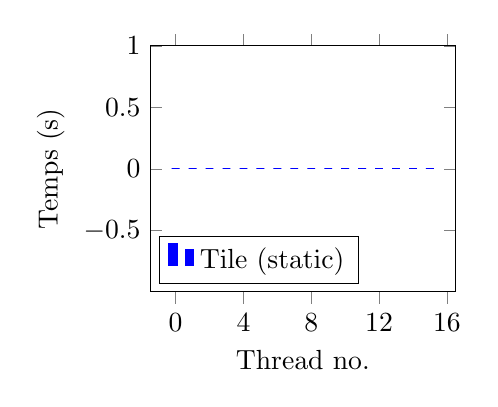
\begin{tikzpicture}
\begin{axis}[
  ybar,
  bar width=0.1cm,
  xlabel={Thread no.},
  ylabel={Temps (s)},
  ymin=0,
  legend pos=south west,
  width=0.45\textwidth,
  xtick distance=4
]

% Données pour le premier graphique (à gauche)
\addplot[color=blue, fill=blue] coordinates {
  (0,0.000000) (1,0.000000) (2,0.000000) (3,0.000000) (4,0.000000) (5,0.000000) (6,0.000000) (7,0.000000) (8,0.000000) (9,0.000000) (10,0.000000) (11,0.000000) (12,0.000000) (13,0.000000) (14,0.000000) (15,0.000000)
};
\addlegendentry{Tile (static)}

\end{axis}
\end{tikzpicture}
\hfill
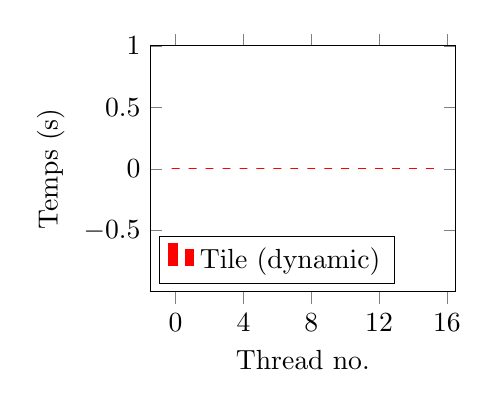
\begin{tikzpicture}
\begin{axis}[
  ybar,
  bar width=0.1cm,
  xlabel={Thread no.},
  ylabel={Temps (s)},
  ymin=,
  legend pos=south west,
  width=0.45\textwidth,
  xtick distance=4
]

% Données pour le deuxième graphique (au milieu)
\addplot[color=red, fill=red] coordinates {
  (0,0.000000) (1,0.000000) (2,0.000000) (3,0.000000) (4,0.000000) (5,0.000000) (6,0.000000) (7,0.000000) (8,0.000000) (9,0.000000) (10,0.000000) (11,0.000000) (12,0.000000) (13,0.000000) (14,0.000000) (15,0.000000)
};
\addlegendentry{Tile (dynamic)}

\end{axis}
\end{tikzpicture}
\hfill
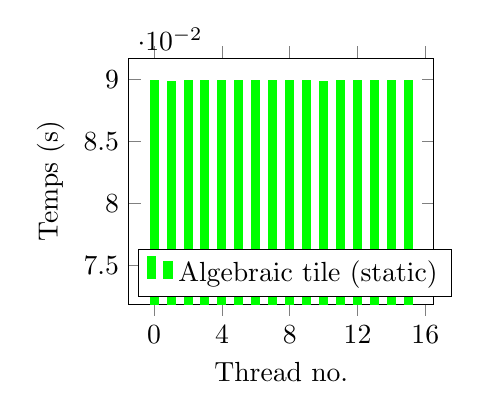
\begin{tikzpicture}
\begin{axis}[
  ybar,
  bar width=0.1cm,
  xlabel={Thread no.},
  ylabel={Temps (s)},
  ymin=.071895,
  legend pos=south west,
  width=0.45\textwidth,
  xtick distance=4
]

% Données pour le troisième graphique (à droite)
\addplot[color=green, fill=green] coordinates {
  (0,0.089903) (1,0.089877) (2,0.089922) (3,0.089921) (4,0.089909) (5,0.089895) (6,0.089891) (7,0.089879) (8,0.089900) (9,0.089881) (10,0.089869) (11,0.089923) (12,0.089900) (13,0.089913) (14,0.089916) (15,0.089916)
};
\addlegendentry{Algebraic tile (static)}

\end{axis}
\end{tikzpicture}

\caption{Temps d'exécution des threads pour le fichier symm.c}
\label{fig:graphes}
\end{figure}

\begin{table}[htbp]
  \centering
  \caption{Statistiques pour le fichier symm.c}
  \begin{tabular}{|c|c|c|c|}
    \hline
    Statistique & Algebraic Tile & Tile (static) & Tile (dynamic) \\ 
    \hline
    Skewness (g1)  & -0.366726 &  &  \\ 
    Kurtosis (g2)  & -1.12189 &  &  \\ 
    Coefficient de variation $ \frac{\sigma}{\overline{x}} $ & 0.000188789 &  & \\ 
    Percent Imbalance metric en \% & 0.0245826 &  & \\ 
    Coefficient de Gini  & 0.000107193 &  & \\ 
    Temps d'exécution (s) &  1.983352    &  4.185306   &  4.463861   \\ 

    \hline
  \end{tabular}
\end{table}\newline
g1=$ \frac{\sum_{i=1}^{n} (x_i - \overline{x})^3}{n\sigma^3} $\
g2=$ \frac{\sum_{i=1}^{n} (x_i - \overline{x})^4}{n\sigma^4} $\
Coefficient de Gini = $ \frac{\sum_{i=1}^{n}\sum_{j=1}^{n} |x_i - x_j|}{2n^2\overline{x}} $\
\newpage

\begin{figure}
\centering

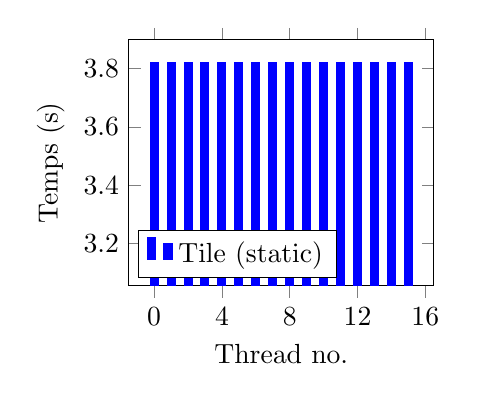
\begin{tikzpicture}
\begin{axis}[
  ybar,
  bar width=0.1cm,
  xlabel={Thread no.},
  ylabel={Temps (s)},
  ymin=3.055819,
  legend pos=south west,
  width=0.45\textwidth,
  xtick distance=4
]

% Données pour le premier graphique (à gauche)
\addplot[color=blue, fill=blue] coordinates {
  (0,3.821341) (1,3.819774) (2,3.819906) (3,3.819838) (4,3.819996) (5,3.819967) (6,3.820159) (7,3.820044) (8,3.820028) (9,3.820095) (10,3.819911) (11,3.819934) (12,3.821787) (13,3.821728) (14,3.821716) (15,3.819912)
};
\addlegendentry{Tile (static)}

\end{axis}
\end{tikzpicture}
\hfill
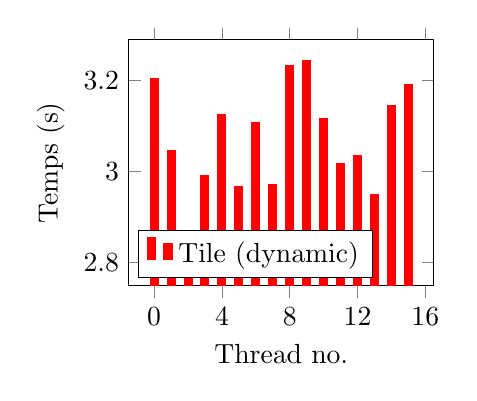
\begin{tikzpicture}
\begin{axis}[
  ybar,
  bar width=0.1cm,
  xlabel={Thread no.},
  ylabel={Temps (s)},
  ymin=,
  legend pos=south west,
  width=0.45\textwidth,
  xtick distance=4
]

% Données pour le deuxième graphique (au milieu)
\addplot[color=red, fill=red] coordinates {
  (0,3.205459) (1,3.044981) (2,2.793017) (3,2.991881) (4,3.124348) (5,2.966205) (6,3.107606) (7,2.970936) (8,3.232290) (9,3.245048) (10,3.116770) (11,3.017089) (12,3.035811) (13,2.949759) (14,3.145588) (15,3.191189)
};
\addlegendentry{Tile (dynamic)}

\end{axis}
\end{tikzpicture}
\hfill
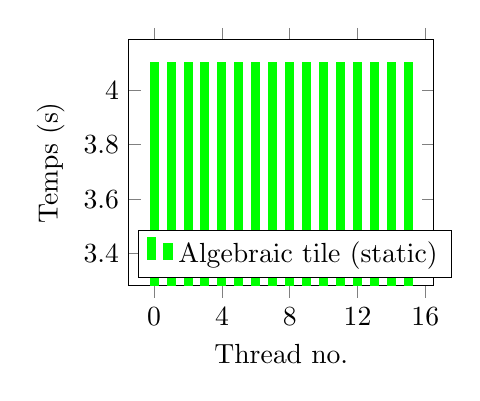
\begin{tikzpicture}
\begin{axis}[
  ybar,
  bar width=0.1cm,
  xlabel={Thread no.},
  ylabel={Temps (s)},
  ymin=3.281975,
  legend pos=south west,
  width=0.45\textwidth,
  xtick distance=4
]

% Données pour le troisième graphique (à droite)
\addplot[color=green, fill=green] coordinates {
  (0,4.102601) (1,4.102649) (2,4.102546) (3,4.102541) (4,4.102604) (5,4.102574) (6,4.102602) (7,4.102469) (8,4.102741) (9,4.102546) (10,4.102620) (11,4.102471) (12,4.102656) (13,4.102621) (14,4.102536) (15,4.102773)
};
\addlegendentry{Algebraic tile (static)}

\end{axis}
\end{tikzpicture}

\caption{Temps d'exécution des threads pour le fichier syr2k.c}
\label{fig:graphes}
\end{figure}

\begin{table}[htbp]
  \centering
  \caption{Statistiques pour le fichier syr2k.c}
  \begin{tabular}{|c|c|c|c|}
    \hline
    Statistique & Algebraic Tile & Tile (static) & Tile (dynamic) \\ 
    \hline
    Skewness (g1)  & 0.486025 & 1.1493 & -0.445512 \\ 
    Kurtosis (g2)  & -0.0831041 & -0.544706 & -0.263013 \\ 
    Coefficient de variation $ \frac{\sigma}{\overline{x}} $ & 1.96459e-05 & 0.000193165 & 0.0385895\\ 
    Percent Imbalance metric en \% & 0.00421684 & 0.0368288 & 5.66334\\ 
    Coefficient de Gini  & 1.08049e-05 & 9.23725e-05 & 0.0216039\\ 
    Temps d'exécution (s) &  4.102986    &  3.822449   &  3.246426   \\ 

    \hline
  \end{tabular}
\end{table}\newline
g1=$ \frac{\sum_{i=1}^{n} (x_i - \overline{x})^3}{n\sigma^3} $\
g2=$ \frac{\sum_{i=1}^{n} (x_i - \overline{x})^4}{n\sigma^4} $\
Coefficient de Gini = $ \frac{\sum_{i=1}^{n}\sum_{j=1}^{n} |x_i - x_j|}{2n^2\overline{x}} $\
\newpage

\begin{figure}
\centering

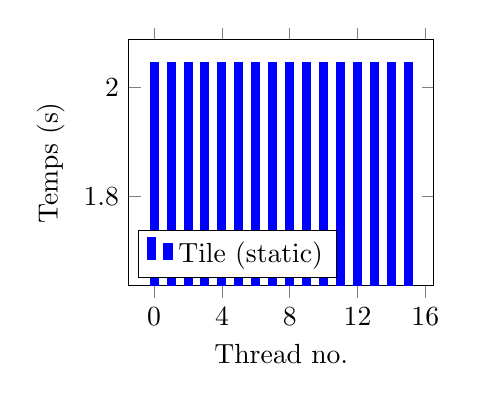
\begin{tikzpicture}
\begin{axis}[
  ybar,
  bar width=0.1cm,
  xlabel={Thread no.},
  ylabel={Temps (s)},
  ymin=1.636492,
  legend pos=south west,
  width=0.45\textwidth,
  xtick distance=4
]

% Données pour le premier graphique (à gauche)
\addplot[color=blue, fill=blue] coordinates {
  (0,2.045759) (1,2.045615) (2,2.045679) (3,2.045724) (4,2.045677) (5,2.045707) (6,2.045657) (7,2.045623) (8,2.045717) (9,2.045754) (10,2.045721) (11,2.045743) (12,2.045773) (13,2.045671) (14,2.045658) (15,2.045716)
};
\addlegendentry{Tile (static)}

\end{axis}
\end{tikzpicture}
\hfill
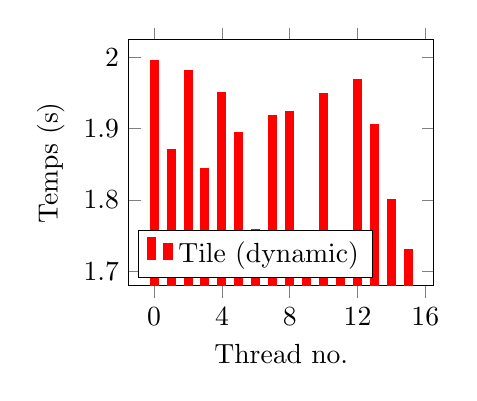
\begin{tikzpicture}
\begin{axis}[
  ybar,
  bar width=0.1cm,
  xlabel={Thread no.},
  ylabel={Temps (s)},
  ymin=,
  legend pos=south west,
  width=0.45\textwidth,
  xtick distance=4
]

% Données pour le deuxième graphique (au milieu)
\addplot[color=red, fill=red] coordinates {
  (0,1.995701) (1,1.871101) (2,1.981217) (3,1.844060) (4,1.950053) (5,1.893893) (6,1.758797) (7,1.917726) (8,1.923666) (9,1.708169) (10,1.948804) (11,1.728077) (12,1.968511) (13,1.905538) (14,1.799924) (15,1.729934)
};
\addlegendentry{Tile (dynamic)}

\end{axis}
\end{tikzpicture}
\hfill
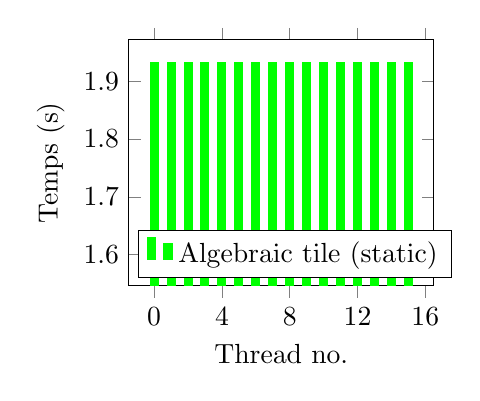
\begin{tikzpicture}
\begin{axis}[
  ybar,
  bar width=0.1cm,
  xlabel={Thread no.},
  ylabel={Temps (s)},
  ymin=1.546104,
  legend pos=south west,
  width=0.45\textwidth,
  xtick distance=4
]

% Données pour le troisième graphique (à droite)
\addplot[color=green, fill=green] coordinates {
  (0,1.932702) (1,1.932735) (2,1.932792) (3,1.932726) (4,1.932722) (5,1.932716) (6,1.932679) (7,1.932705) (8,1.932767) (9,1.932820) (10,1.932690) (11,1.932881) (12,1.932631) (13,1.932716) (14,1.932767) (15,1.932713)
};
\addlegendentry{Algebraic tile (static)}

\end{axis}
\end{tikzpicture}

\caption{Temps d'exécution des threads pour le fichier syrk.c}
\label{fig:graphes}
\end{figure}

\begin{table}[htbp]
  \centering
  \caption{Statistiques pour le fichier syrk.c}
  \begin{tabular}{|c|c|c|c|}
    \hline
    Statistique & Algebraic Tile & Tile (static) & Tile (dynamic) \\ 
    \hline
    Skewness (g1)  & 0.805506 & -0.237468 & -0.457212 \\ 
    Kurtosis (g2)  & 0.674426 & -0.928159 & -1.19616 \\ 
    Coefficient de variation $ \frac{\sigma}{\overline{x}} $ & 2.98515e-05 & 2.24549e-05 & 0.0502601\\ 
    Percent Imbalance metric en \% & 0.00729534 & 0.00356846 & 6.70372\\ 
    Coefficient de Gini  & 1.59061e-05 & 1.27631e-05 & 0.0282813\\ 
    Temps d'exécution (s) &  1.933104    &  2.045912   &  1.996480   \\ 

    \hline
  \end{tabular}
\end{table}\newline
g1=$ \frac{\sum_{i=1}^{n} (x_i - \overline{x})^3}{n\sigma^3} $\
g2=$ \frac{\sum_{i=1}^{n} (x_i - \overline{x})^4}{n\sigma^4} $\
Coefficient de Gini = $ \frac{\sum_{i=1}^{n}\sum_{j=1}^{n} |x_i - x_j|}{2n^2\overline{x}} $\
\newpage

\begin{figure}
\centering

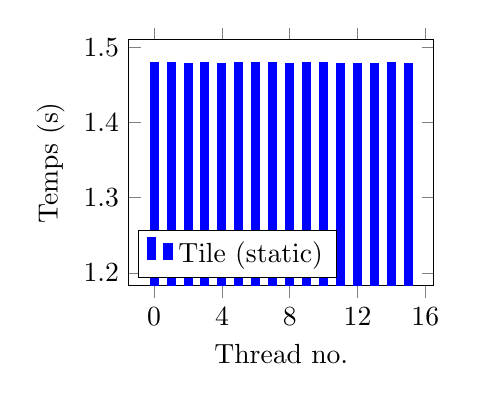
\begin{tikzpicture}
\begin{axis}[
  ybar,
  bar width=0.1cm,
  xlabel={Thread no.},
  ylabel={Temps (s)},
  ymin=1.182933,
  legend pos=south west,
  width=0.45\textwidth,
  xtick distance=4
]

% Données pour le premier graphique (à gauche)
\addplot[color=blue, fill=blue] coordinates {
  (0,1.480022) (1,1.478869) (2,1.478700) (3,1.479078) (4,1.478722) (5,1.478999) (6,1.478957) (7,1.478917) (8,1.478778) (9,1.480066) (10,1.480024) (11,1.478760) (12,1.478667) (13,1.478825) (14,1.478979) (15,1.478671)
};
\addlegendentry{Tile (static)}

\end{axis}
\end{tikzpicture}
\hfill
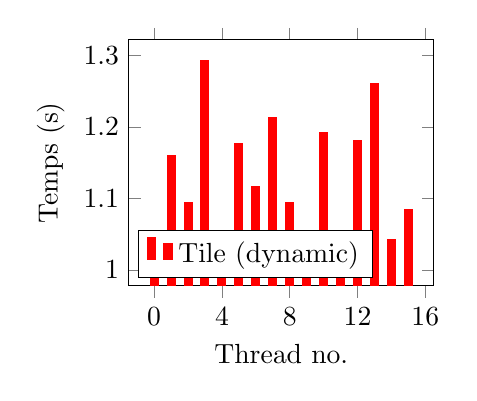
\begin{tikzpicture}
\begin{axis}[
  ybar,
  bar width=0.1cm,
  xlabel={Thread no.},
  ylabel={Temps (s)},
  ymin=,
  legend pos=south west,
  width=0.45\textwidth,
  xtick distance=4
]

% Données pour le deuxième graphique (au milieu)
\addplot[color=red, fill=red] coordinates {
  (0,1.049981) (1,1.159536) (2,1.094180) (3,1.293010) (4,1.017604) (5,1.176667) (6,1.115963) (7,1.212967) (8,1.094588) (9,1.037061) (10,1.192032) (11,1.006652) (12,1.180753) (13,1.261031) (14,1.043117) (15,1.084181)
};
\addlegendentry{Tile (dynamic)}

\end{axis}
\end{tikzpicture}
\hfill
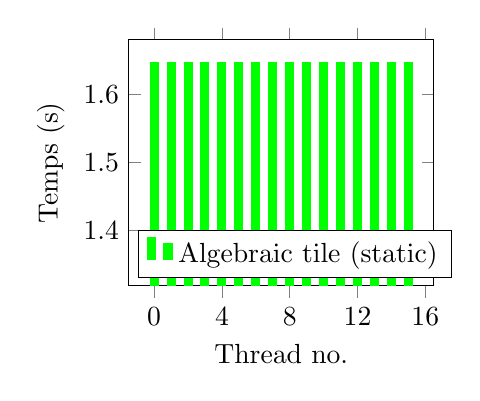
\begin{tikzpicture}
\begin{axis}[
  ybar,
  bar width=0.1cm,
  xlabel={Thread no.},
  ylabel={Temps (s)},
  ymin=1.318000,
  legend pos=south west,
  width=0.45\textwidth,
  xtick distance=4
]

% Données pour le troisième graphique (à droite)
\addplot[color=green, fill=green] coordinates {
  (0,1.647627) (1,1.647596) (2,1.647635) (3,1.647504) (4,1.647710) (5,1.647674) (6,1.647541) (7,1.647594) (8,1.647504) (9,1.647521) (10,1.647552) (11,1.647651) (12,1.647574) (13,1.647561) (14,1.647632) (15,1.647500)
};
\addlegendentry{Algebraic tile (static)}

\end{axis}
\end{tikzpicture}

\caption{Temps d'exécution des threads pour le fichier trmm.c}
\label{fig:graphes}
\end{figure}

\begin{table}[htbp]
  \centering
  \caption{Statistiques pour le fichier trmm.c}
  \begin{tabular}{|c|c|c|c|}
    \hline
    Statistique & Algebraic Tile & Tile (static) & Tile (dynamic) \\ 
    \hline
    Skewness (g1)  & 0.251292 & 1.37965 & 0.358652 \\ 
    Kurtosis (g2)  & -0.982396 & 0.232279 & -0.960662 \\ 
    Coefficient de variation $ \frac{\sigma}{\overline{x}} $ & 3.80027e-05 & 0.00032596 & 0.0753238\\ 
    Percent Imbalance metric en \% & 0.00728337 & 0.0680162 & 14.8107\\ 
    Coefficient de Gini  & 2.167e-05 & 0.000156988 & 0.042768\\ 
    Temps d'exécution (s) &  1.647963    &  1.480536   &  1.293560   \\ 

    \hline
  \end{tabular}
\end{table}\newline
g1=$ \frac{\sum_{i=1}^{n} (x_i - \overline{x})^3}{n\sigma^3} $\
g2=$ \frac{\sum_{i=1}^{n} (x_i - \overline{x})^4}{n\sigma^4} $\
Coefficient de Gini = $ \frac{\sum_{i=1}^{n}\sum_{j=1}^{n} |x_i - x_j|}{2n^2\overline{x}} $\
\newpage

\begin{figure}
\centering

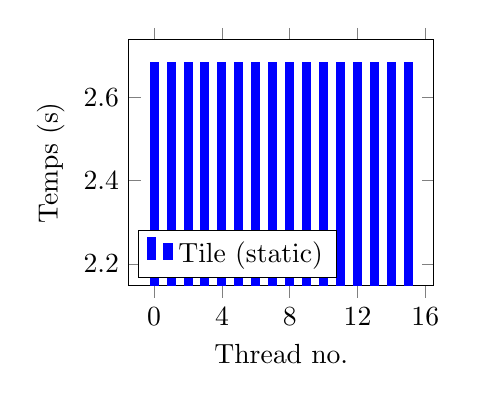
\begin{tikzpicture}
\begin{axis}[
  ybar,
  bar width=0.1cm,
  xlabel={Thread no.},
  ylabel={Temps (s)},
  ymin=2.147588,
  legend pos=south west,
  width=0.45\textwidth,
  xtick distance=4
]

% Données pour le premier graphique (à gauche)
\addplot[color=blue, fill=blue] coordinates {
  (0,2.684538) (1,2.684509) (2,2.684525) (3,2.684520) (4,2.684503) (5,2.684515) (6,2.684485) (7,2.684518) (8,2.684509) (9,2.684512) (10,2.684653) (11,2.684532) (12,2.684504) (13,2.684505) (14,2.684513) (15,2.684542)
};
\addlegendentry{Tile (static)}

\end{axis}
\end{tikzpicture}
\hfill
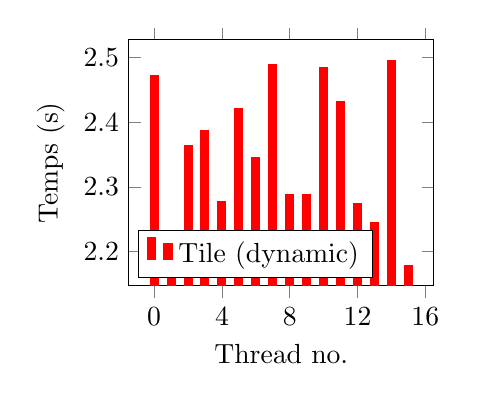
\begin{tikzpicture}
\begin{axis}[
  ybar,
  bar width=0.1cm,
  xlabel={Thread no.},
  ylabel={Temps (s)},
  ymin=,
  legend pos=south west,
  width=0.45\textwidth,
  xtick distance=4
]

% Données pour le deuxième graphique (au milieu)
\addplot[color=red, fill=red] coordinates {
  (0,2.472980) (1,2.200281) (2,2.363815) (3,2.387550) (4,2.276784) (5,2.420554) (6,2.345253) (7,2.489817) (8,2.288373) (9,2.288528) (10,2.484317) (11,2.431773) (12,2.274510) (13,2.244227) (14,2.496002) (15,2.178509)
};
\addlegendentry{Tile (dynamic)}

\end{axis}
\end{tikzpicture}
\hfill
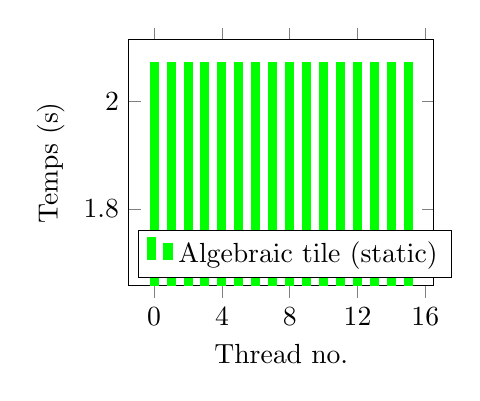
\begin{tikzpicture}
\begin{axis}[
  ybar,
  bar width=0.1cm,
  xlabel={Thread no.},
  ylabel={Temps (s)},
  ymin=1.657333,
  legend pos=south west,
  width=0.45\textwidth,
  xtick distance=4
]

% Données pour le troisième graphique (à droite)
\addplot[color=green, fill=green] coordinates {
  (0,2.071987) (1,2.072182) (2,2.071667) (3,2.071802) (4,2.071842) (5,2.072034) (6,2.071857) (7,2.071753) (8,2.072363) (9,2.071818) (10,2.071752) (11,2.071978) (12,2.072206) (13,2.072011) (14,2.072129) (15,2.072044)
};
\addlegendentry{Algebraic tile (static)}

\end{axis}
\end{tikzpicture}

\caption{Temps d'exécution des threads pour le fichier 2mm.c}
\label{fig:graphes}
\end{figure}

\begin{table}[htbp]
  \centering
  \caption{Statistiques pour le fichier 2mm.c}
  \begin{tabular}{|c|c|c|c|}
    \hline
    Statistique & Algebraic Tile & Tile (static) & Tile (dynamic) \\ 
    \hline
    Skewness (g1)  & 0.363304 & 2.75467 & -0.0668757 \\ 
    Kurtosis (g2)  & -0.684363 & 7.37766 & -1.28842 \\ 
    Coefficient de variation $ \frac{\sigma}{\overline{x}} $ & 9.01567e-05 & 1.34299e-05 & 0.0436643\\ 
    Percent Imbalance metric en \% & 0.0194502 & 0.00495433 & 6.09096\\ 
    Coefficient de Gini  & 5.09348e-05 & 5.57449e-06 & 0.0249298\\ 
    Temps d'exécution (s) &  2.073075    &  2.684839   &  2.499211   \\ 

    \hline
  \end{tabular}
\end{table}\newline
g1=$ \frac{\sum_{i=1}^{n} (x_i - \overline{x})^3}{n\sigma^3} $\
g2=$ \frac{\sum_{i=1}^{n} (x_i - \overline{x})^4}{n\sigma^4} $\
Coefficient de Gini = $ \frac{\sum_{i=1}^{n}\sum_{j=1}^{n} |x_i - x_j|}{2n^2\overline{x}} $\
\newpage

\begin{figure}
\centering

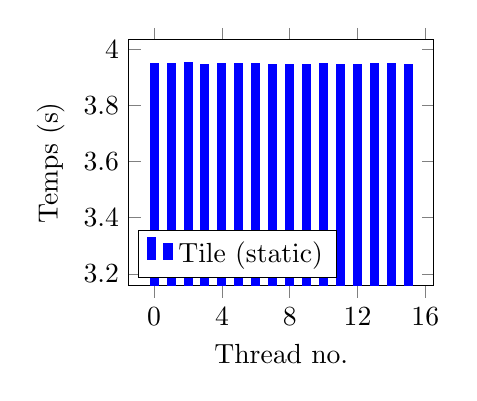
\begin{tikzpicture}
\begin{axis}[
  ybar,
  bar width=0.1cm,
  xlabel={Thread no.},
  ylabel={Temps (s)},
  ymin=3.157652,
  legend pos=south west,
  width=0.45\textwidth,
  xtick distance=4
]

% Données pour le premier graphique (à gauche)
\addplot[color=blue, fill=blue] coordinates {
  (0,3.947387) (1,3.948467) (2,3.954238) (3,3.947329) (4,3.948839) (5,3.947446) (6,3.949399) (7,3.947169) (8,3.947177) (9,3.947076) (10,3.947795) (11,3.947066) (12,3.947148) (13,3.947428) (14,3.948473) (15,3.947178)
};
\addlegendentry{Tile (static)}

\end{axis}
\end{tikzpicture}
\hfill
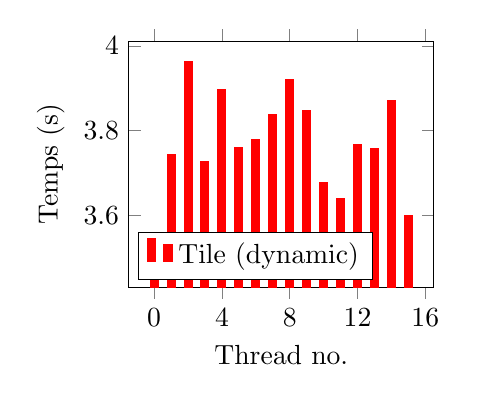
\begin{tikzpicture}
\begin{axis}[
  ybar,
  bar width=0.1cm,
  xlabel={Thread no.},
  ylabel={Temps (s)},
  ymin=,
  legend pos=south west,
  width=0.45\textwidth,
  xtick distance=4
]

% Données pour le deuxième graphique (au milieu)
\addplot[color=red, fill=red] coordinates {
  (0,3.478602) (1,3.742530) (2,3.962786) (3,3.726990) (4,3.896971) (5,3.759993) (6,3.778983) (7,3.837465) (8,3.920239) (9,3.846724) (10,3.677975) (11,3.638935) (12,3.766331) (13,3.757988) (14,3.869799) (15,3.599992)
};
\addlegendentry{Tile (dynamic)}

\end{axis}
\end{tikzpicture}
\hfill
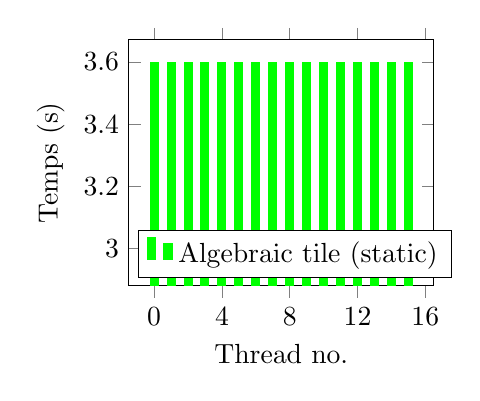
\begin{tikzpicture}
\begin{axis}[
  ybar,
  bar width=0.1cm,
  xlabel={Thread no.},
  ylabel={Temps (s)},
  ymin=2.879168,
  legend pos=south west,
  width=0.45\textwidth,
  xtick distance=4
]

% Données pour le troisième graphique (à droite)
\addplot[color=green, fill=green] coordinates {
  (0,3.599496) (1,3.599488) (2,3.599303) (3,3.599794) (4,3.599075) (5,3.599101) (6,3.599306) (7,3.599017) (8,3.599050) (9,3.599190) (10,3.598976) (11,3.598960) (12,3.598960) (13,3.599208) (14,3.599421) (15,3.599179)
};
\addlegendentry{Algebraic tile (static)}

\end{axis}
\end{tikzpicture}

\caption{Temps d'exécution des threads pour le fichier 3mm.c}
\label{fig:graphes}
\end{figure}

\begin{table}[htbp]
  \centering
  \caption{Statistiques pour le fichier 3mm.c}
  \begin{tabular}{|c|c|c|c|}
    \hline
    Statistique & Algebraic Tile & Tile (static) & Tile (dynamic) \\ 
    \hline
    Skewness (g1)  & 0.892947 & 2.74273 & -0.544609 \\ 
    Kurtosis (g2)  & 0.143217 & 6.97889 & -0.0526179 \\ 
    Coefficient de variation $ \frac{\sigma}{\overline{x}} $ & 6.34676e-05 & 0.000438021 & 0.032413\\ 
    Percent Imbalance metric en \% & 0.0159479 & 0.155467 & 5.21444\\ 
    Coefficient de Gini  & 3.47406e-05 & 0.000178708 & 0.018018\\ 
    Temps d'exécution (s) &  3.600617    &  3.955588   &  4.035524   \\ 

    \hline
  \end{tabular}
\end{table}\newline
g1=$ \frac{\sum_{i=1}^{n} (x_i - \overline{x})^3}{n\sigma^3} $\
g2=$ \frac{\sum_{i=1}^{n} (x_i - \overline{x})^4}{n\sigma^4} $\
Coefficient de Gini = $ \frac{\sum_{i=1}^{n}\sum_{j=1}^{n} |x_i - x_j|}{2n^2\overline{x}} $\
\newpage

\begin{figure}
\centering

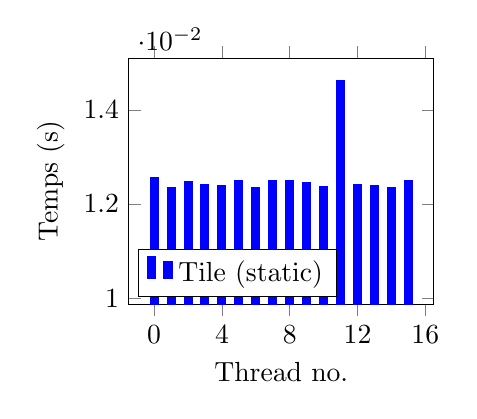
\begin{tikzpicture}
\begin{axis}[
  ybar,
  bar width=0.1cm,
  xlabel={Thread no.},
  ylabel={Temps (s)},
  ymin=.009872,
  legend pos=south west,
  width=0.45\textwidth,
  xtick distance=4
]

% Données pour le premier graphique (à gauche)
\addplot[color=blue, fill=blue] coordinates {
  (0,0.012554) (1,0.012340) (2,0.012483) (3,0.012413) (4,0.012391) (5,0.012509) (6,0.012360) (7,0.012508) (8,0.012506) (9,0.012449) (10,0.012375) (11,0.014625) (12,0.012420) (13,0.012383) (14,0.012358) (15,0.012491)
};
\addlegendentry{Tile (static)}

\end{axis}
\end{tikzpicture}
\hfill
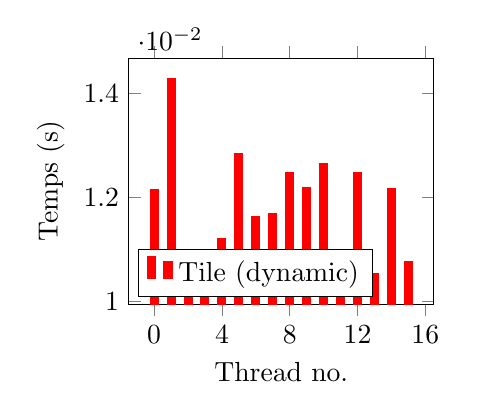
\begin{tikzpicture}
\begin{axis}[
  ybar,
  bar width=0.1cm,
  xlabel={Thread no.},
  ylabel={Temps (s)},
  ymin=,
  legend pos=south west,
  width=0.45\textwidth,
  xtick distance=4
]

% Données pour le deuxième graphique (au milieu)
\addplot[color=red, fill=red] coordinates {
  (0,0.012145) (1,0.014291) (2,0.010451) (3,0.010337) (4,0.011205) (5,0.012845) (6,0.011627) (7,0.011691) (8,0.012476) (9,0.012185) (10,0.012653) (11,0.010522) (12,0.012475) (13,0.010536) (14,0.012167) (15,0.010757)
};
\addlegendentry{Tile (dynamic)}

\end{axis}
\end{tikzpicture}
\hfill
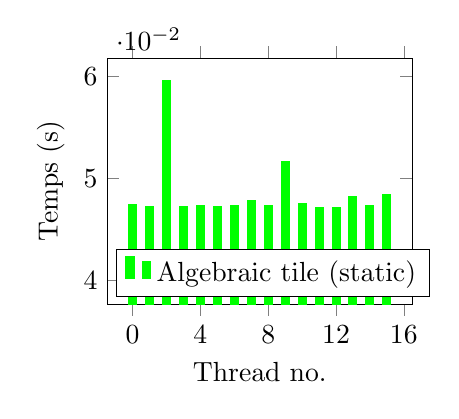
\begin{tikzpicture}
\begin{axis}[
  ybar,
  bar width=0.1cm,
  xlabel={Thread no.},
  ylabel={Temps (s)},
  ymin=.037685,
  legend pos=south west,
  width=0.45\textwidth,
  xtick distance=4
]

% Données pour le troisième graphique (à droite)
\addplot[color=green, fill=green] coordinates {
  (0,0.047422) (1,0.047212) (2,0.059587) (3,0.047269) (4,0.047366) (5,0.047269) (6,0.047339) (7,0.047801) (8,0.047322) (9,0.051641) (10,0.047521) (11,0.047136) (12,0.047107) (13,0.048263) (14,0.047304) (15,0.048383)
};
\addlegendentry{Algebraic tile (static)}

\end{axis}
\end{tikzpicture}

\caption{Temps d'exécution des threads pour le fichier atax.c}
\label{fig:graphes}
\end{figure}

\begin{table}[htbp]
  \centering
  \caption{Statistiques pour le fichier atax.c}
  \begin{tabular}{|c|c|c|c|}
    \hline
    Statistique & Algebraic Tile & Tile (static) & Tile (dynamic) \\ 
    \hline
    Skewness (g1)  & 3.01253 & 3.52685 & 0.440592 \\ 
    Kurtosis (g2)  & 7.93151 & 10.673 & -0.237347 \\ 
    Coefficient de variation $ \frac{\sigma}{\overline{x}} $ & 0.0630113 & 0.0424489 & 0.0901\\ 
    Percent Imbalance metric en \% & 22.8689 & 16.3225 & 21.391\\ 
    Coefficient de Gini  & 0.0219675 & 0.0128188 & 0.0498814\\ 
    Temps d'exécution (s) &  0.060362    &  0.015176   &  0.015002   \\ 

    \hline
  \end{tabular}
\end{table}\newline
g1=$ \frac{\sum_{i=1}^{n} (x_i - \overline{x})^3}{n\sigma^3} $\
g2=$ \frac{\sum_{i=1}^{n} (x_i - \overline{x})^4}{n\sigma^4} $\
Coefficient de Gini = $ \frac{\sum_{i=1}^{n}\sum_{j=1}^{n} |x_i - x_j|}{2n^2\overline{x}} $\
\newpage

\begin{figure}
\centering

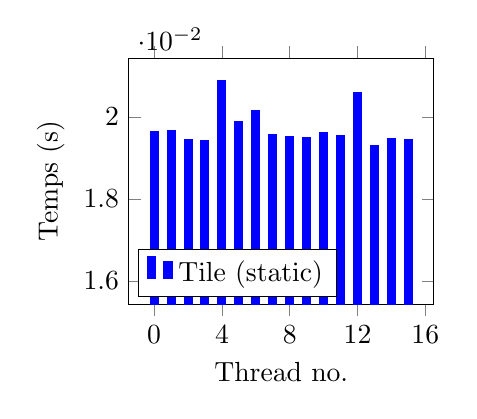
\begin{tikzpicture}
\begin{axis}[
  ybar,
  bar width=0.1cm,
  xlabel={Thread no.},
  ylabel={Temps (s)},
  ymin=.015437,
  legend pos=south west,
  width=0.45\textwidth,
  xtick distance=4
]

% Données pour le premier graphique (à gauche)
\addplot[color=blue, fill=blue] coordinates {
  (0,0.019654) (1,0.019671) (2,0.019453) (3,0.019419) (4,0.020890) (5,0.019877) (6,0.020168) (7,0.019562) (8,0.019522) (9,0.019493) (10,0.019611) (11,0.019536) (12,0.020596) (13,0.019297) (14,0.019473) (15,0.019459)
};
\addlegendentry{Tile (static)}

\end{axis}
\end{tikzpicture}
\hfill
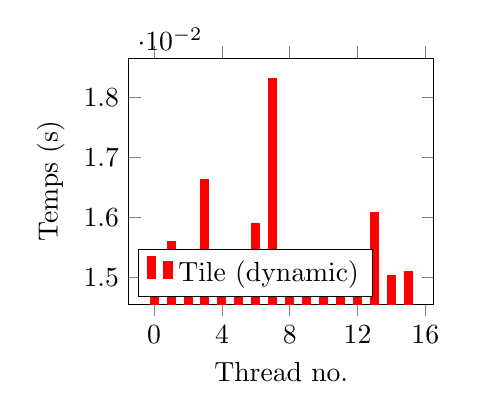
\begin{tikzpicture}
\begin{axis}[
  ybar,
  bar width=0.1cm,
  xlabel={Thread no.},
  ylabel={Temps (s)},
  ymin=,
  legend pos=south west,
  width=0.45\textwidth,
  xtick distance=4
]

% Données pour le deuxième graphique (au milieu)
\addplot[color=red, fill=red] coordinates {
  (0,0.015390) (1,0.015599) (2,0.015105) (3,0.016627) (4,0.015214) (5,0.014907) (6,0.015901) (7,0.018312) (8,0.014900) (9,0.014981) (10,0.015323) (11,0.014968) (12,0.015020) (13,0.016084) (14,0.015039) (15,0.015108)
};
\addlegendentry{Tile (dynamic)}

\end{axis}
\end{tikzpicture}
\hfill
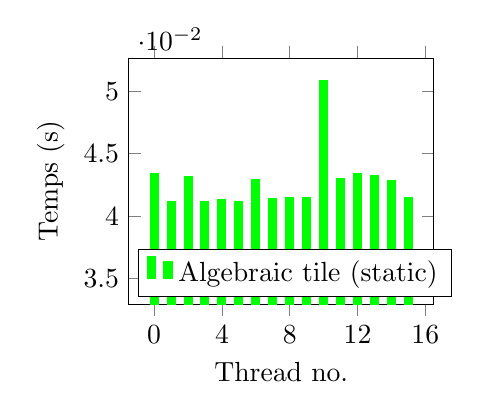
\begin{tikzpicture}
\begin{axis}[
  ybar,
  bar width=0.1cm,
  xlabel={Thread no.},
  ylabel={Temps (s)},
  ymin=.032956,
  legend pos=south west,
  width=0.45\textwidth,
  xtick distance=4
]

% Données pour le troisième graphique (à droite)
\addplot[color=green, fill=green] coordinates {
  (0,0.043398) (1,0.041199) (2,0.043187) (3,0.041203) (4,0.041339) (5,0.041195) (6,0.042916) (7,0.041386) (8,0.041465) (9,0.041461) (10,0.050865) (11,0.042975) (12,0.043404) (13,0.043219) (14,0.042893) (15,0.041460)
};
\addlegendentry{Algebraic tile (static)}

\end{axis}
\end{tikzpicture}

\caption{Temps d'exécution des threads pour le fichier bicg.c}
\label{fig:graphes}
\end{figure}

\begin{table}[htbp]
  \centering
  \caption{Statistiques pour le fichier bicg.c}
  \begin{tabular}{|c|c|c|c|}
    \hline
    Statistique & Algebraic Tile & Tile (static) & Tile (dynamic) \\ 
    \hline
    Skewness (g1)  & 2.73336 & 1.61108 & 2.14635 \\ 
    Kurtosis (g2)  & 7.21997 & 1.40981 & 4.12413 \\ 
    Coefficient de variation $ \frac{\sigma}{\overline{x}} $ & 0.0533895 & 0.02194 & 0.0553375\\ 
    Percent Imbalance metric en \% & 19.0582 & 5.87883 & 17.9145\\ 
    Coefficient de Gini  & 0.0220128 & 0.010554 & 0.0253201\\ 
    Temps d'exécution (s) &  0.051523    &  0.023340   &  0.019864   \\ 

    \hline
  \end{tabular}
\end{table}\newline
g1=$ \frac{\sum_{i=1}^{n} (x_i - \overline{x})^3}{n\sigma^3} $\
g2=$ \frac{\sum_{i=1}^{n} (x_i - \overline{x})^4}{n\sigma^4} $\
Coefficient de Gini = $ \frac{\sum_{i=1}^{n}\sum_{j=1}^{n} |x_i - x_j|}{2n^2\overline{x}} $\
\newpage

\begin{figure}
\centering

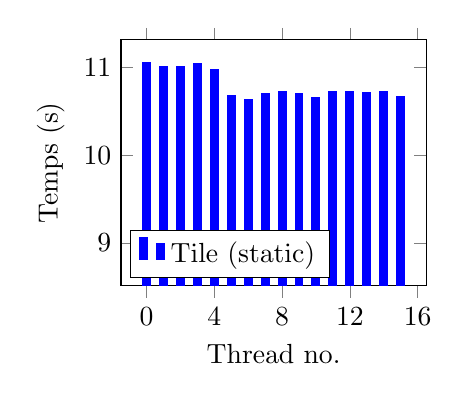
\begin{tikzpicture}
\begin{axis}[
  ybar,
  bar width=0.1cm,
  xlabel={Thread no.},
  ylabel={Temps (s)},
  ymin=8.511480,
  legend pos=south west,
  width=0.45\textwidth,
  xtick distance=4
]

% Données pour le premier graphique (à gauche)
\addplot[color=blue, fill=blue] coordinates {
  (0,11.062070) (1,11.008313) (2,11.013789) (3,11.049967) (4,10.979229) (5,10.685760) (6,10.639351) (7,10.699473) (8,10.728288) (9,10.700110) (10,10.652799) (11,10.725340) (12,10.723639) (13,10.716046) (14,10.728440) (15,10.672221)
};
\addlegendentry{Tile (static)}

\end{axis}
\end{tikzpicture}
\hfill
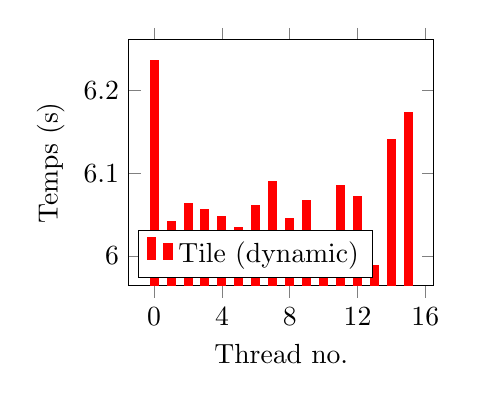
\begin{tikzpicture}
\begin{axis}[
  ybar,
  bar width=0.1cm,
  xlabel={Thread no.},
  ylabel={Temps (s)},
  ymin=,
  legend pos=south west,
  width=0.45\textwidth,
  xtick distance=4
]

% Données pour le deuxième graphique (au milieu)
\addplot[color=red, fill=red] coordinates {
  (0,6.236957) (1,6.041426) (2,6.063909) (3,6.055693) (4,6.047318) (5,6.033736) (6,6.061107) (7,6.089917) (8,6.045357) (9,6.066532) (10,6.025305) (11,6.085779) (12,6.071295) (13,5.988590) (14,6.140585) (15,6.173608)
};
\addlegendentry{Tile (dynamic)}

\end{axis}
\end{tikzpicture}
\hfill
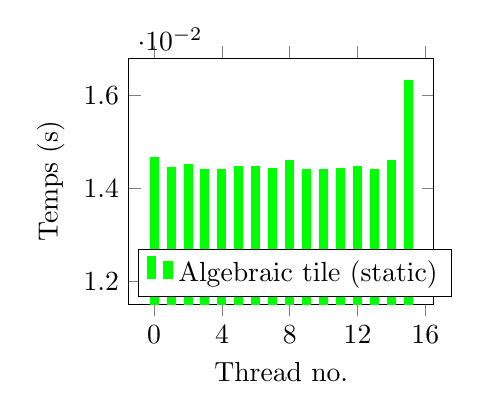
\begin{tikzpicture}
\begin{axis}[
  ybar,
  bar width=0.1cm,
  xlabel={Thread no.},
  ylabel={Temps (s)},
  ymin=.011516,
  legend pos=south west,
  width=0.45\textwidth,
  xtick distance=4
]

% Données pour le troisième graphique (à droite)
\addplot[color=green, fill=green] coordinates {
  (0,0.014665) (1,0.014443) (2,0.014504) (3,0.014400) (4,0.014396) (5,0.014466) (6,0.014469) (7,0.014423) (8,0.014594) (9,0.014400) (10,0.014402) (11,0.014419) (12,0.014461) (13,0.014412) (14,0.014608) (15,0.016317)
};
\addlegendentry{Algebraic tile (static)}

\end{axis}
\end{tikzpicture}

\caption{Temps d'exécution des threads pour le fichier doitgen.c}
\label{fig:graphes}
\end{figure}

\begin{table}[htbp]
  \centering
  \caption{Statistiques pour le fichier doitgen.c}
  \begin{tabular}{|c|c|c|c|}
    \hline
    Statistique & Algebraic Tile & Tile (static) & Tile (dynamic) \\ 
    \hline
    Skewness (g1)  & 3.4305 & 0.759765 & 1.29966 \\ 
    Kurtosis (g2)  & 10.2144 & -1.23859 & 1.32049 \\ 
    Coefficient de variation $ \frac{\sigma}{\overline{x}} $ & 0.0311256 & 0.0142336 & 0.00971248\\ 
    Percent Imbalance metric en \% & 11.866 & 2.43511 & 2.63741\\ 
    Coefficient de Gini  & 0.00999367 & 0.00734387 & 0.00495191\\ 
    Temps d'exécution (s) &  0.016759    &  16.277046   &  12.066926   \\ 

    \hline
  \end{tabular}
\end{table}\newline
g1=$ \frac{\sum_{i=1}^{n} (x_i - \overline{x})^3}{n\sigma^3} $\
g2=$ \frac{\sum_{i=1}^{n} (x_i - \overline{x})^4}{n\sigma^4} $\
Coefficient de Gini = $ \frac{\sum_{i=1}^{n}\sum_{j=1}^{n} |x_i - x_j|}{2n^2\overline{x}} $\
\newpage

\begin{figure}
\centering

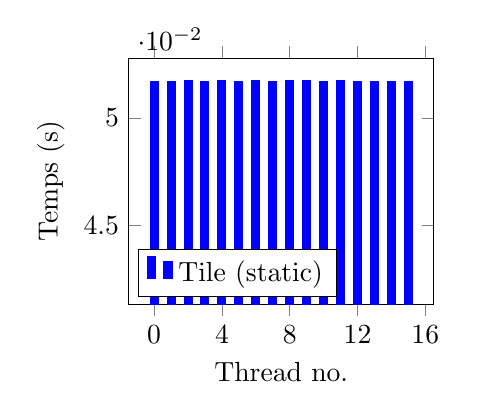
\begin{tikzpicture}
\begin{axis}[
  ybar,
  bar width=0.1cm,
  xlabel={Thread no.},
  ylabel={Temps (s)},
  ymin=.041351,
  legend pos=south west,
  width=0.45\textwidth,
  xtick distance=4
]

% Données pour le premier graphique (à gauche)
\addplot[color=blue, fill=blue] coordinates {
  (0,0.051691) (1,0.051707) (2,0.051717) (3,0.051707) (4,0.051726) (5,0.051693) (6,0.051738) (7,0.051689) (8,0.051714) (9,0.051717) (10,0.051689) (11,0.051720) (12,0.051707) (13,0.051693) (14,0.051705) (15,0.051704)
};
\addlegendentry{Tile (static)}

\end{axis}
\end{tikzpicture}
\hfill
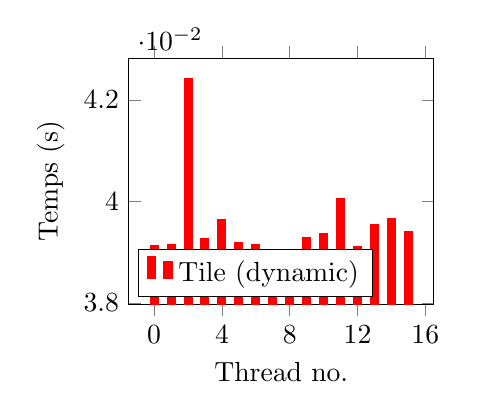
\begin{tikzpicture}
\begin{axis}[
  ybar,
  bar width=0.1cm,
  xlabel={Thread no.},
  ylabel={Temps (s)},
  ymin=,
  legend pos=south west,
  width=0.45\textwidth,
  xtick distance=4
]

% Données pour le deuxième graphique (au milieu)
\addplot[color=red, fill=red] coordinates {
  (0,0.039127) (1,0.039146) (2,0.042422) (3,0.039277) (4,0.039645) (5,0.039179) (6,0.039144) (7,0.038937) (8,0.038378) (9,0.039293) (10,0.039358) (11,0.040061) (12,0.039108) (13,0.039550) (14,0.039672) (15,0.039400)
};
\addlegendentry{Tile (dynamic)}

\end{axis}
\end{tikzpicture}
\hfill
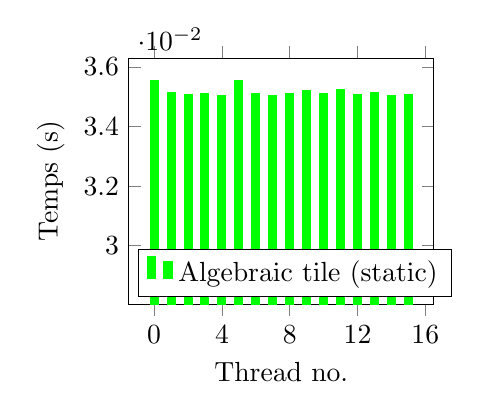
\begin{tikzpicture}
\begin{axis}[
  ybar,
  bar width=0.1cm,
  xlabel={Thread no.},
  ylabel={Temps (s)},
  ymin=.028032,
  legend pos=south west,
  width=0.45\textwidth,
  xtick distance=4
]

% Données pour le troisième graphique (à droite)
\addplot[color=green, fill=green] coordinates {
  (0,0.035549) (1,0.035150) (2,0.035082) (3,0.035121) (4,0.035044) (5,0.035544) (6,0.035111) (7,0.035043) (8,0.035096) (9,0.035204) (10,0.035113) (11,0.035243) (12,0.035061) (13,0.035152) (14,0.035040) (15,0.035083)
};
\addlegendentry{Algebraic tile (static)}

\end{axis}
\end{tikzpicture}

\caption{Temps d'exécution des threads pour le fichier mvt.c}
\label{fig:graphes}
\end{figure}

\begin{table}[htbp]
  \centering
  \caption{Statistiques pour le fichier mvt.c}
  \begin{tabular}{|c|c|c|c|}
    \hline
    Statistique & Algebraic Tile & Tile (static) & Tile (dynamic) \\ 
    \hline
    Skewness (g1)  & 1.75837 & 0.405388 & 2.53709 \\ 
    Kurtosis (g2)  & 1.78945 & -0.529204 & 6.68478 \\ 
    Coefficient de variation $ \frac{\sigma}{\overline{x}} $ & 0.00438822 & 0.000266904 & 0.0212355\\ 
    Percent Imbalance metric en \% & 1.09257 & 0.0593727 & 7.44888\\ 
    Coefficient de Gini  & 0.00205795 & 0.000149202 & 0.00898403\\ 
    Temps d'exécution (s) &  0.035910    &  0.051824   &  0.042575   \\ 

    \hline
  \end{tabular}
\end{table}\newline
g1=$ \frac{\sum_{i=1}^{n} (x_i - \overline{x})^3}{n\sigma^3} $\
g2=$ \frac{\sum_{i=1}^{n} (x_i - \overline{x})^4}{n\sigma^4} $\
Coefficient de Gini = $ \frac{\sum_{i=1}^{n}\sum_{j=1}^{n} |x_i - x_j|}{2n^2\overline{x}} $\
\newpage

\begin{figure}
\centering

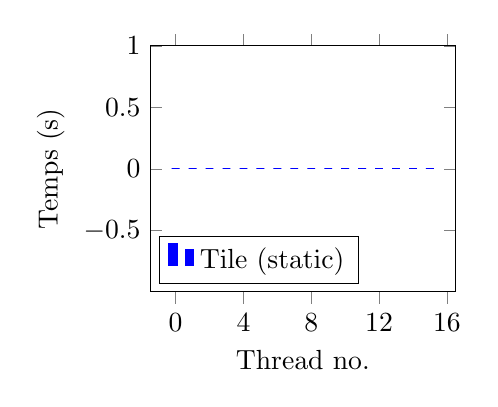
\begin{tikzpicture}
\begin{axis}[
  ybar,
  bar width=0.1cm,
  xlabel={Thread no.},
  ylabel={Temps (s)},
  ymin=0,
  legend pos=south west,
  width=0.45\textwidth,
  xtick distance=4
]

% Données pour le premier graphique (à gauche)
\addplot[color=blue, fill=blue] coordinates {
  (0,0.000000) (1,0.000000) (2,0.000000) (3,0.000000) (4,0.000000) (5,0.000000) (6,0.000000) (7,0.000000) (8,0.000000) (9,0.000000) (10,0.000000) (11,0.000000) (12,0.000000) (13,0.000000) (14,0.000000) (15,0.000000)
};
\addlegendentry{Tile (static)}

\end{axis}
\end{tikzpicture}
\hfill
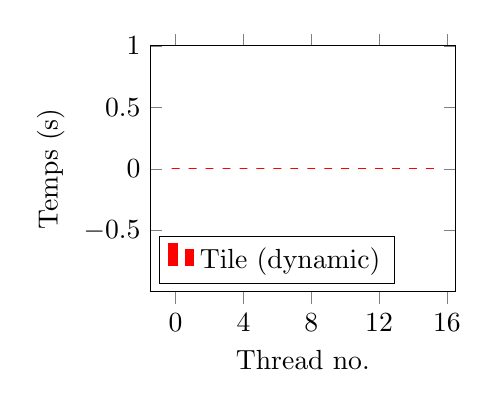
\begin{tikzpicture}
\begin{axis}[
  ybar,
  bar width=0.1cm,
  xlabel={Thread no.},
  ylabel={Temps (s)},
  ymin=,
  legend pos=south west,
  width=0.45\textwidth,
  xtick distance=4
]

% Données pour le deuxième graphique (au milieu)
\addplot[color=red, fill=red] coordinates {
  (0,0.000000) (1,0.000000) (2,0.000000) (3,0.000000) (4,0.000000) (5,0.000000) (6,0.000000) (7,0.000000) (8,0.000000) (9,0.000000) (10,0.000000) (11,0.000000) (12,0.000000) (13,0.000000) (14,0.000000) (15,0.000000)
};
\addlegendentry{Tile (dynamic)}

\end{axis}
\end{tikzpicture}
\hfill
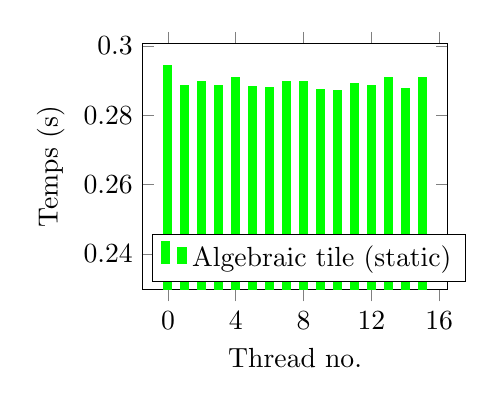
\begin{tikzpicture}
\begin{axis}[
  ybar,
  bar width=0.1cm,
  xlabel={Thread no.},
  ylabel={Temps (s)},
  ymin=.229743,
  legend pos=south west,
  width=0.45\textwidth,
  xtick distance=4
]

% Données pour le troisième graphique (à droite)
\addplot[color=green, fill=green] coordinates {
  (0,0.294201) (1,0.288604) (2,0.289665) (3,0.288548) (4,0.290832) (5,0.288399) (6,0.287933) (7,0.289800) (8,0.289816) (9,0.287312) (10,0.287179) (11,0.289076) (12,0.288496) (13,0.290815) (14,0.287655) (15,0.290940)
};
\addlegendentry{Algebraic tile (static)}

\end{axis}
\end{tikzpicture}

\caption{Temps d'exécution des threads pour le fichier durbin.c}
\label{fig:graphes}
\end{figure}

\begin{table}[htbp]
  \centering
  \caption{Statistiques pour le fichier durbin.c}
  \begin{tabular}{|c|c|c|c|}
    \hline
    Statistique & Algebraic Tile & Tile (static) & Tile (dynamic) \\ 
    \hline
    Skewness (g1)  & 1.20553 &  &  \\ 
    Kurtosis (g2)  & 1.46505 &  &  \\ 
    Coefficient de variation $ \frac{\sigma}{\overline{x}} $ & 0.00595962 &  & \\ 
    Percent Imbalance metric en \% & 1.6839 &  & \\ 
    Coefficient de Gini  & 0.0031544 &  & \\ 
    Temps d'exécution (s) &  0.441350    &  0.004166   &  0.003990   \\ 

    \hline
  \end{tabular}
\end{table}\newline
g1=$ \frac{\sum_{i=1}^{n} (x_i - \overline{x})^3}{n\sigma^3} $\
g2=$ \frac{\sum_{i=1}^{n} (x_i - \overline{x})^4}{n\sigma^4} $\
Coefficient de Gini = $ \frac{\sum_{i=1}^{n}\sum_{j=1}^{n} |x_i - x_j|}{2n^2\overline{x}} $\
\newpage

\begin{figure}
\centering

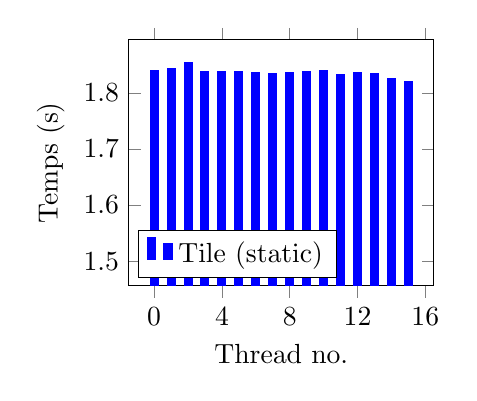
\begin{tikzpicture}
\begin{axis}[
  ybar,
  bar width=0.1cm,
  xlabel={Thread no.},
  ylabel={Temps (s)},
  ymin=1.456046,
  legend pos=south west,
  width=0.45\textwidth,
  xtick distance=4
]

% Données pour le premier graphique (à gauche)
\addplot[color=blue, fill=blue] coordinates {
  (0,1.839898) (1,1.842444) (2,1.854717) (3,1.837056) (4,1.837846) (5,1.837292) (6,1.836349) (7,1.835196) (8,1.836817) (9,1.837852) (10,1.839050) (11,1.833256) (12,1.835831) (13,1.833633) (14,1.825779) (15,1.820058)
};
\addlegendentry{Tile (static)}

\end{axis}
\end{tikzpicture}
\hfill
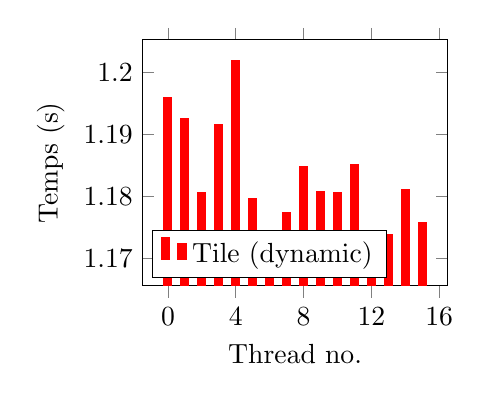
\begin{tikzpicture}
\begin{axis}[
  ybar,
  bar width=0.1cm,
  xlabel={Thread no.},
  ylabel={Temps (s)},
  ymin=,
  legend pos=south west,
  width=0.45\textwidth,
  xtick distance=4
]

% Données pour le deuxième graphique (au milieu)
\addplot[color=red, fill=red] coordinates {
  (0,1.196016) (1,1.192625) (2,1.180580) (3,1.191637) (4,1.202012) (5,1.179598) (6,1.168872) (7,1.177457) (8,1.184882) (9,1.180836) (10,1.180679) (11,1.185148) (12,1.170151) (13,1.173886) (14,1.181040) (15,1.175726)
};
\addlegendentry{Tile (dynamic)}

\end{axis}
\end{tikzpicture}
\hfill
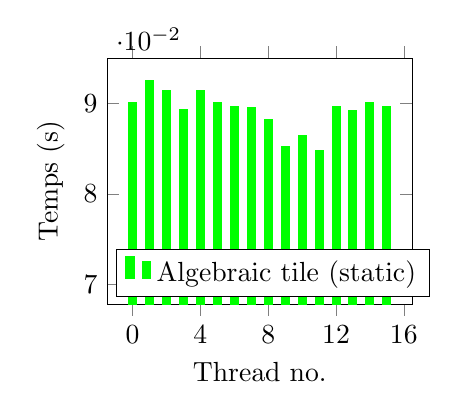
\begin{tikzpicture}
\begin{axis}[
  ybar,
  bar width=0.1cm,
  xlabel={Thread no.},
  ylabel={Temps (s)},
  ymin=.067828,
  legend pos=south west,
  width=0.45\textwidth,
  xtick distance=4
]

% Données pour le troisième graphique (à droite)
\addplot[color=green, fill=green] coordinates {
  (0,0.090086) (1,0.092558) (2,0.091418) (3,0.089395) (4,0.091410) (5,0.090094) (6,0.089694) (7,0.089612) (8,0.088196) (9,0.085200) (10,0.086457) (11,0.084786) (12,0.089624) (13,0.089277) (14,0.090122) (15,0.089650)
};
\addlegendentry{Algebraic tile (static)}

\end{axis}
\end{tikzpicture}

\caption{Temps d'exécution des threads pour le fichier gramschmidt.c}
\label{fig:graphes}
\end{figure}

\begin{table}[htbp]
  \centering
  \caption{Statistiques pour le fichier gramschmidt.c}
  \begin{tabular}{|c|c|c|c|}
    \hline
    Statistique & Algebraic Tile & Tile (static) & Tile (dynamic) \\ 
    \hline
    Skewness (g1)  & -0.809457 & 0.12782 & 0.525736 \\ 
    Kurtosis (g2)  & 0.0170044 & 2.00392 & -0.402158 \\ 
    Coefficient de variation $ \frac{\sigma}{\overline{x}} $ & 0.0231666 & 0.00384092 & 0.00752215\\ 
    Percent Imbalance metric en \% & 3.73701 & 0.995241 & 1.64405\\ 
    Coefficient de Gini  & 0.0122006 & 0.00189327 & 0.00417677\\ 
    Temps d'exécution (s) &  0.140977 &  2.041889   &  1.524002   \\ 

    \hline
  \end{tabular}
\end{table}\newline
g1=$ \frac{\sum_{i=1}^{n} (x_i - \overline{x})^3}{n\sigma^3} $\
g2=$ \frac{\sum_{i=1}^{n} (x_i - \overline{x})^4}{n\sigma^4} $\
Coefficient de Gini = $ \frac{\sum_{i=1}^{n}\sum_{j=1}^{n} |x_i - x_j|}{2n^2\overline{x}} $\
\newpage

  \end{document}
